\section{Introduction}
\label{introduction}

\emph{The performance and execution time of data-driven control systems depends on the data being processed.}

The various tasks in a control system, and in particular the state estimation task, will have an execution time that depends heavily on the current data.
For example, an autonomous robot equipped with a camera needs to self-localize by processing, among other things, the video feed. 
The robot tries to detect and track known objects in the frames to determine its current position.
The amount of time this visually-guided estimator will take to process each frame depends on the contents of the frame [???], as well as on the settings used for the computer vision algorithms.
To guarantee that the control objectives are achieved, the system is typically over-engineered to complete, in a timely manner, all computation and control tasks based on a Worst-Case estimate of their Execution Time (WCET).

Whether computed offline [??] or online \cite{hendsethB12_OnlineWCET} the WCET generally provides a pessimistic view of system performance.
That's because in many cases, worst-case runtimes are not typical of the system's operation. 
I.e., worst-case is not the average case. 
To illustrate this point, consider the execution times shown in Fig.~\ref{fig:time_ecdf} for a self-localization algorithm which we study in Section \ref{delayErrorCurve}.
It can be seen that the average can differ significantly from the worst-case.
Since computation time typically correlates with consumed energy, much energy is therefore wasted on computations that are not necessary for the current data input.
\todo[inline]{HA: Yash, plz change the axis on fig \figref{fig:time_ecdf} from ns to ms or sec}
\begin{figure}[t]
\centering
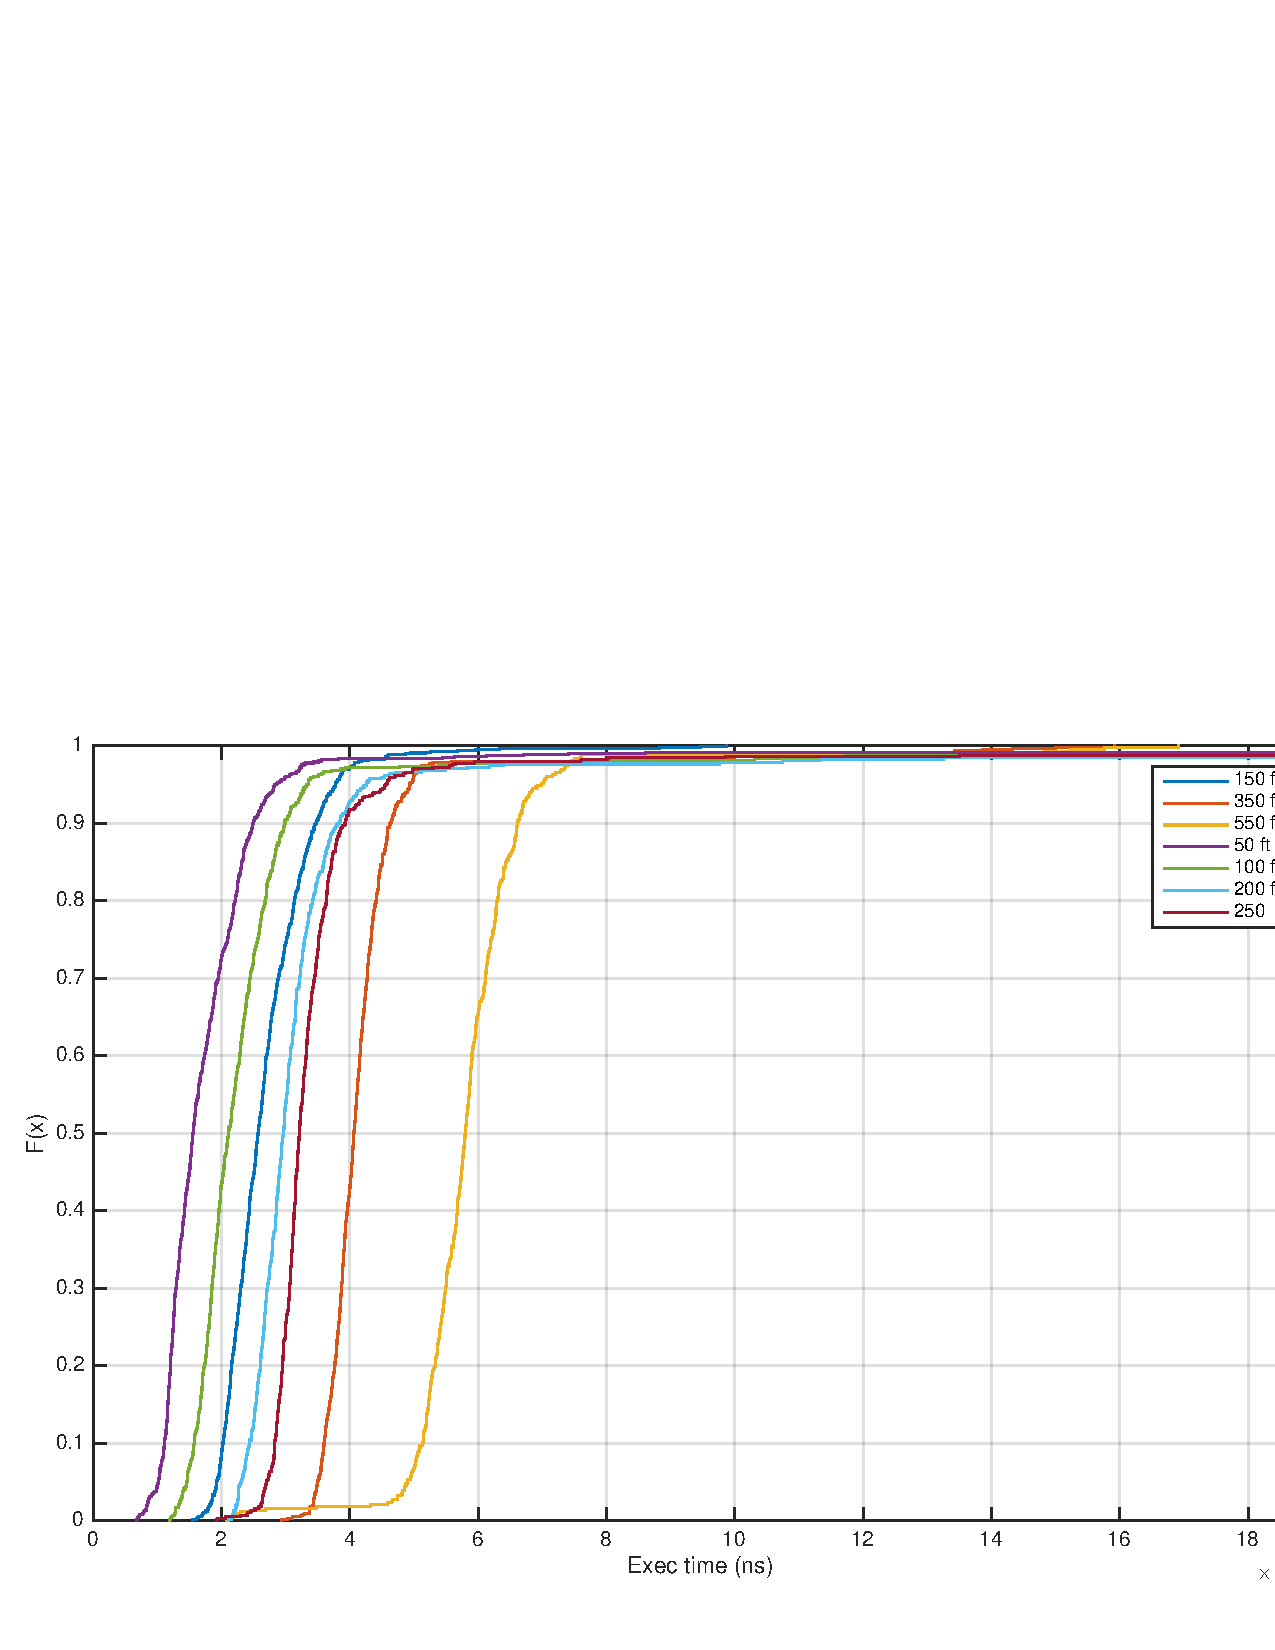
\includegraphics[width=0.7\linewidth]{figures/time_ecdf}
\caption{Cumulative Distribution Function $F(x)$ for the execution time of a visually guided self-localization algorithm, obtained at different settings of the algorithm. The variability in times is captured by the spread of the CDF.}
\label{fig:time_ecdf}
\end{figure}

In this paper we focus on the execution time of state estimators used in control systems.
While prior work leverages the \emph{inherent} data-dependent variability of certain algorithms' execution time to do ??? [???], in this paper, we \emph{introduce} variability into the execution time, guided by the fact that the best estimates are not always required for good control performance.
Rather, the control algorithm can decide, based on its objectives, what quality of state estimate is sufficient at the current time step.
\todo[inline]{HA: was it the right choice then to start by talking about data-dependent variability? doesn't seem relevant to what we do.}
Since computation time and energy are usually negatively correlated with quality of estimate, choosing a poorer quality estimate where appropriate usually results in energy savings.

Specifically, we investigate the design of robust controllers with the use of contract-based state estimation algorithms.

Our contributions: 
the formulation and solution of an RMPC problem where the controller receives noisy state estimates from a contract-based estimation algorithm.
\\
a procedure to make any perception tool chain contract-based 
\\
set computations? or are those borrowed from [14]?


\begin{figure}[t]
	\centering
	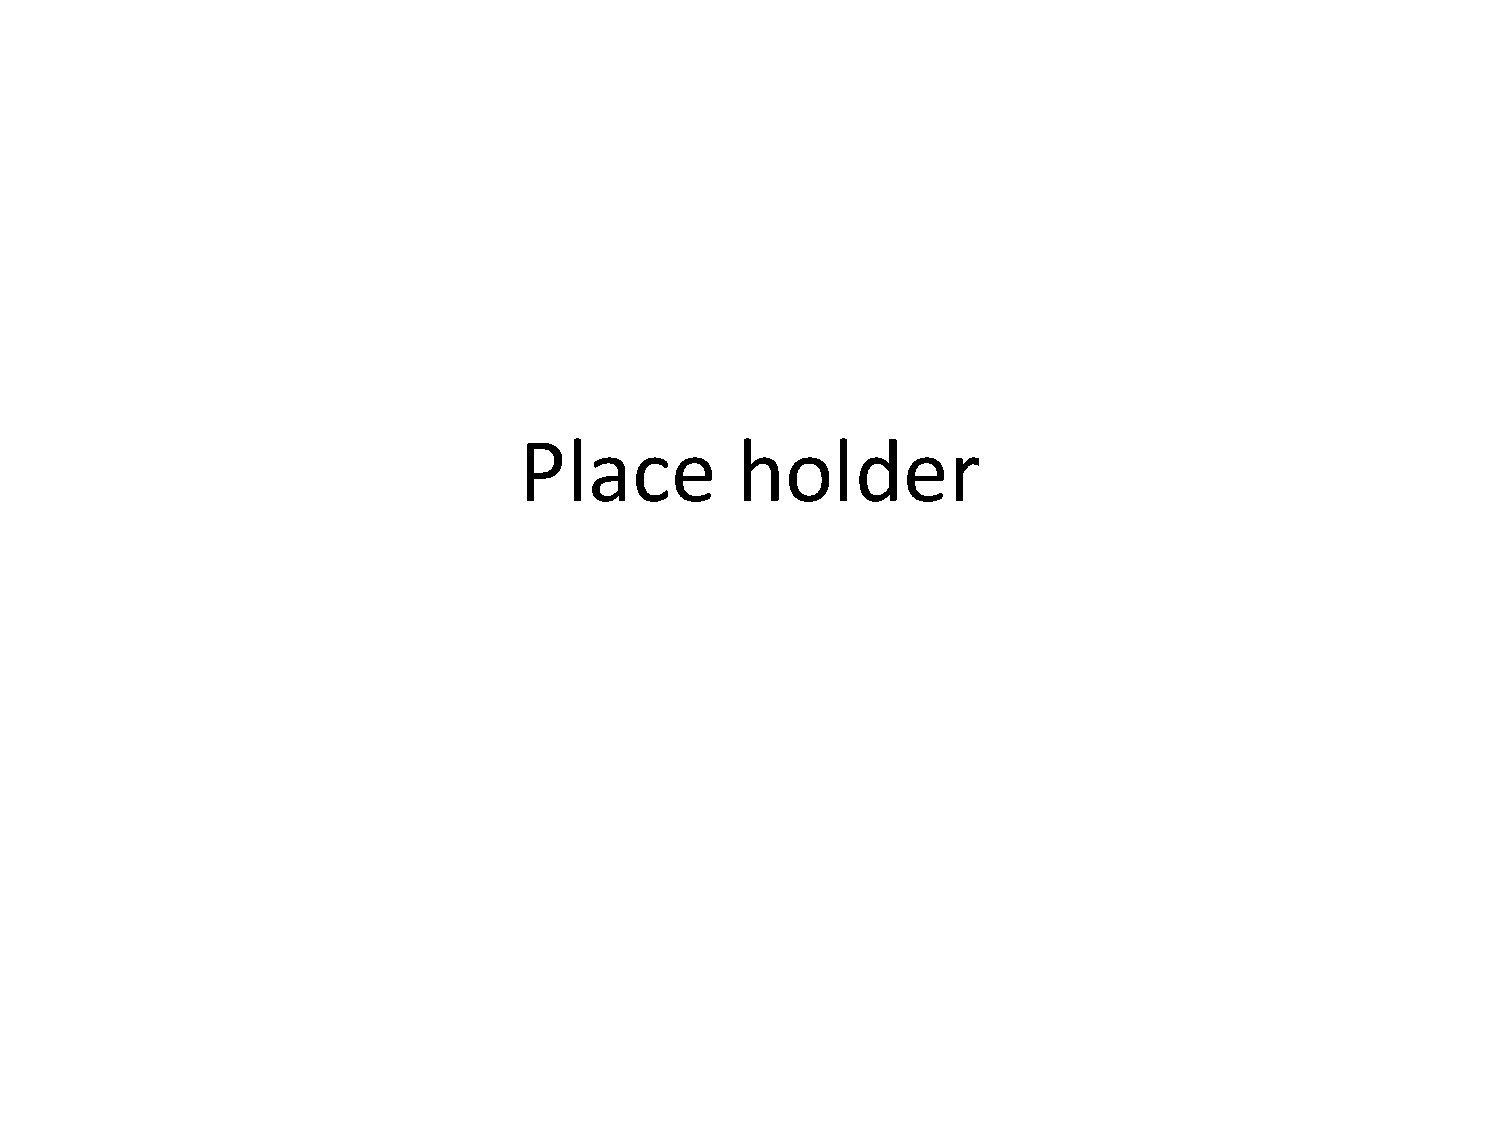
\includegraphics[width=0.7\linewidth]{figures/placeHolder}
	\caption{Control with anytime estimation}
	\label{fig:feedbackloop}
\end{figure}